\documentclass[10pt]{article}
\makeatletter
\usepackage[numbered,autolinebreaks,useliterate]{mcode}
\usepackage{textcomp}
\usepackage{verbatim}
\usepackage{lmodern}
\usepackage{comment}
\excludecomment{Answ}
\usepackage{listings}
\usepackage{color} %red, green, blue, yellow, cyan, magenta, black, white
\definecolor{mygreen}{RGB}{28,172,0} % color values Red, Green, Blue
\definecolor{mylilas}{RGB}{170,55,241}
\renewcommand\paragraph{\@startsection{paragraph}{4}{\z@}%
            {-2.5ex\@plus -1ex \@minus -.25ex}%
            {1.25ex \@plus .25ex}%
            {\normalfont\normalsize\bfseries}}
\makeatother
\usepackage{gensymb}
\setcounter{secnumdepth}{4}
\usepackage{amsmath}
%\usepackage{mathtools}
\usepackage{graphicx}
\usepackage{slashed}
\usepackage{lineno}
\usepackage{latexsym}
\usepackage{subfigure}
\usepackage{amssymb}
\newtheorem{thm}{Theorem}[section]
\newtheorem{cor}[thm]{Corollary}
\newtheorem{lem}[thm]{Lemma}
\usepackage[numbers,sort]{natbib}
\usepackage{enumerate}
\newcommand{\bb}{\begin{equation}}
\newcommand{\ee}{\end{equation}}
\newtheorem{defin}{Definition}
\usepackage{multirow}
\usepackage{ctable}
\usepackage{bm}
\usepackage{enumerate}
\newcommand{\D}[2]{\frac{\partial #1}{\partial #2}}
\newcommand{\DD}[2]{\frac{\partial^2 #1}{\partial #2^2}}
\newcommand{\UB}[2]{\underbrace{#1}_{\textrm{\parbox{8em}{\centering #2}}}}
\newcommand{\rd}{\text{ d}}
\newcommand{\disk}{}
\usepackage{framed}
\newcommand{\see}[1]{(see Figure \ref{#1})}
\newcommand{\fig}[1]{Figure \ref{#1}}
\newcommand{\figs}[2]{figures \ref{#1} and \ref{#2}}
\newcommand{\sect}[1]{Section \ref{#1}}
\newcommand{\app}[1]{Appendix \ref{#1}}
\newcommand{\chap}[1]{Chapter \ref{#1}}
\newcommand{\eqn}[1]{equation \eqref{#1}}
\newcommand{\eqns}[2]{equations \eqref{#1} and \eqref{#2}}
\newcommand{\eqnto}[2]{equations \eqref{#1}-\eqref{#2}}
%\usepackage{authblk}
\usepackage{url}
\usepackage{hyperref}
\usepackage{soul}
\newcommand{\eg}{\emph{e.g.} }
\newcommand{\bn}{\bm{n}}
\newcommand{\bu}{\bm{u}}
\newcommand{\ie}{\emph{i.e.} }
\newcommand{\Chapter}[1]{\chapter{#1}\label{#1}}
\newcommand{\Section}[1]{\section{#1}\label{#1}}
\newcommand{\Subsection}[1]{\subsection{#1}\label{#1}}
\newcommand{\Subsubsection}[1]{\subsubsection{#1}\label{#1}}
\newcommand{\Appendix}[1]{\appendix{#1}\label{#1}}
\usepackage[margin=1.5cm,centering]{geometry}
\usepackage[geometry]{ifsym}
\makeatletter
\newcommand\restr[2]{{% we make the whole thing an ordinary symbol
  \left.\kern-\nulldelimiterspace % automatically resize the bar with \right
  #1 % the function
  \vphantom{\big|} % pretend it's a little taller at normal size
  \right|_{#2} % this is the delimiter
  }}
\def\url@leostyle{%
  \@ifundefined{selectfont}{\def\UrlFont{\sf}}{\def\UrlFont{\small\ttfamily}}}
\makeatother
\urlstyle{leo}
\usepackage{multirow}
\usepackage{blkarray}
\usepackage{soul}
\usepackage{framed}
\usepackage{color}
\usepackage{setspace}
\newcommand{\ttttp}{.24\textwidth}
\newcommand{\tttp}{.32\textwidth}
\newcommand{\ttp}{.45\textwidth}
\newcommand{\tp}{.8\textwidth}
\newcommand{\tbo}{.6\textwidth}
 \usepackage[T1]{fontenc}
\usepackage[utf8]{inputenc}
\usepackage{authblk}
 \renewcommand{\l}{\left(}
\renewcommand{\r}{\right)}
%\begin{figure}[h!!!tb]
%\centering
%\subfigure[\label{Godzilla}]{\includegraphics[height=0.35\textwidth]{./Pictures/Godzilla_final_bw.png}}
%\subfigure[\label{Jaeger}]{\includegraphics[height=0.35\textwidth]{./Pictures/Jaeger_finish_bw.png}}
%\caption{\label{Monsters} The two types of monster we are going to consider are: (a) the naturally occurring Kaijus and (b) the man-made Jaegers.}
%\end{figure}
\newcounter{Counter1}

\begin{document}

\lstset{language=Matlab,%
    %basicstyle=\color{red},
    breaklines=true,%
    morekeywords={matlab2tikz},
    keywordstyle=\color{blue},%
    morekeywords=[2]{1}, keywordstyle=[2]{\color{black}},
    identifierstyle=\color{black},%
    stringstyle=\color{mylilas},
    commentstyle=\color{mygreen},%
    showstringspaces=false,%without this there will be a symbol in the places where there is a space
    numbers=left,%
    numberstyle={\tiny \color{black}},% size of the numbers
    numbersep=9pt, % this defines how far the numbers are from the text
    emph=[1]{for,end,break},emphstyle=[1]\color{red}, %some words to emphasise
    %emph=[2]{word1,word2}, emphstyle=[2]{style},    
}


\title{Problem sheet 4}
\author{Thomas E. Woolley\\Last edited on:}
\maketitle
\section{French flag threshold}\label{French flag threshold}
Consider an empty one-dimensional domain, $[0,L]$, such that $x=0$ is insulated. At time $t=0$ the boundary $x=L$ is turned into a source of morphogen, $M$, of constant strength $S$. The morphogen is able to diffuse away from the boundary at a rate $D$ and decays at a rate proportional to itself with constant of proportionality $r$.
\begin{enumerate}
\item Justify the following model of this set up,
\bb
\D{M}{t}=D\DD{M}{x}-rM,\quad 0<x<L,\label{Diffusion}
\ee\bb
M(x,0)=0,
\ee\bb
\D{M(0,t)}{x}=0,\quad M(L,t)=S.
\ee

\item Determine the steady state distribution, $M(x,t)=M_s(x)$.
\setcounter{Counter1}{\value{enumi}}
\end{enumerate}

Suppose the domain is filled with cells that are able to sense the concentration of $M$ and that the cells can differentiate into two different forms based on the concentration of $M$ that they sense. Namely, if $M_s<S/2$ then cells differentiate into form 1, whilst if $M_s>S/2$ then then cells differentiate into form 2. Define $x_s\in[0,L]$ to be the point which delineates the regions between cells of form 1 and cells of form 2.
\begin{enumerate}
\setcounter{enumi}{\value{Counter1}}
\item Draw two sketches of $M_s(x)$ to show that $x_s$ may, or may not exist.\label{skectchxs}

\item Show that
\bb
x_s=\sqrt{\frac{D}{r}}\cosh^{-1}\l\frac{1}{2}\cosh\l\sqrt{\frac{r}{D}}L\r \r.\label{xs}
\ee

\item Using \eqn{xs} and the intuition from question \ref{skectchxs}, under what parameter conditions does $x_s$ exist?  Hint: the inverse of  $\cosh$ does not output real values for all input values.

\item By sketching $M_s$ for multiple values of $L$, suggest what happens to $x_s$ as $L$ gets larger.\label{Sketchxs}

\item Follow the proceeding steps derive a first order approximation of $x_s$ in $L$, for large $L$.
\begin{enumerate}
\item Noting that: 
\begin{itemize}
\item $\cosh(x)=\frac{1}{2}\l\exp(x)+\exp(-x)\r$;
\item $\cosh^{-1}(x)=\ln\l x+\sqrt{x^2-1}\r.$
\end{itemize}
what is $\cosh\l L\sqrt{r/D}\r$ for large $L$?\label{LargeL}

\item Using the answer from part \ref{LargeL} show that, for large $L$,
\bb
x_s\approx\sqrt{\frac{D}{r}}\ln\l\frac{1}{2}\exp\l{\sqrt{\frac{r}{D}}L}\r\r.\label{xs_approx}
\ee
\item Rearrange \eqn{xs_approx} to generate a form
\bb
x_s\approx L-C,\label{Constant_diff}
\ee
where $C$ is a positive constant that should be defined.
\end{enumerate}


\item Does solution \eqref{Constant_diff} confirm the intuition gained from the question \ref{Sketchxs}?

\item What does \eqn{Constant_diff} mean for the cell populations on a large domain?

\item (Optional) Using computer software you are comfortable with plot \eqns{xs}{Constant_diff} with values $D=10$ and $r=1$ for $0\leq L \leq 10$. Be careful of where the solution becomes $x_s$ becomes imaginary. How good is the approximation? Estimate the length, $L$, at which $M_s$ is always above $S/2$.
\end{enumerate}


\begin{Answ}
\subsection{Answers}
\begin{enumerate}
\item 

\bb
\UB{\D{M}{t}}{Rate of change of morphogen concentration}=\UB{D\DD{M}{x}}{Diffusion of morphogen through domain}-\UB{rM}{Decay of morphogen},\quad \UB{0<x<L}{Domain size},
\ee\bb
\UB{M(x,0)=0}{Initial condition},
\ee\bb
\UB{\D{M(0,t)}{x}=0}{Left boundary is insulated},\quad \UB{M(L,t)=S}{Right boundary is a constant flux}.
\ee

\item Since we are looking for a steady state distribution we can set the time derivative to zero. We then look for solutions of the form
\bb
M_s=\exp(\lambda x)\label{exp}
\ee
and derive a condition for $\lambda$. However, in this case it is easier to look for solutions using the substitution
\bb
M_s=A\cosh(\lambda x)+B\sinh(\lambda x),\label{cosh}
\ee
which is simply an alternate form of substitution \eqref{exp}.
Critically, starting with the boundary condition at $x=0$ we find that $B=0$. Similarly, the boundary condition at $x=L$ provides us with
\bb
A=\frac{S}{\cosh(\lambda L)}.
\ee
Finally, substituting \eqn{cosh} into \eqn{Diffusion} and simplifying we generate
\bb
0=D\lambda^2-r.
\ee
Since $\cosh$ is a even function (\ie $f(x)=f(-x)$) we only need to take the positive root. Thus,
\bb
M_s=\frac{S\cosh\l \sqrt{\frac{r}{D}} x\r}{\cosh\l \sqrt{\frac{r}{D}} L\r}.
\ee


\item See \fig{Gradient_plot}. Key things to note, the plot is a $\cosh$, so, it looks approximately exponential. We have to obey the boundary conditions, so the derivative is zero at $x=0$ and the concentration is fixed at $S$ at $x=L$. The final point to note depends on the level of $M_s$ at $x=0$. Depending how steep the gradient and how big $L$ is $x_s$ may, or may not, exist.
\begin{figure}[h!!!tb]
\centering
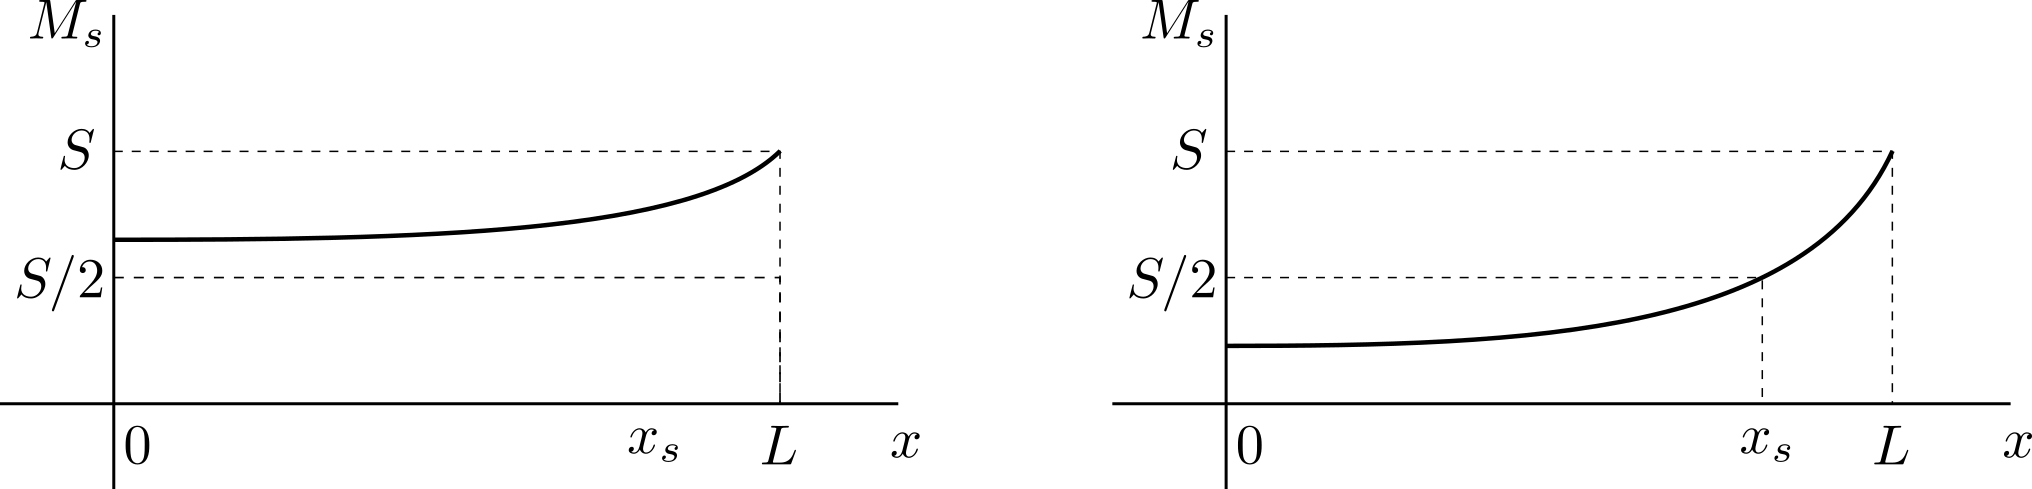
\includegraphics[width=\textwidth]{../../Pictures/Gradient_plot.png}
\caption{\label{Gradient_plot} Sketches of $M_s$ and $x_s$. Note it is possible that the gradient is very shallow (left) and, thus, no $x_s$ exists. However, if the gradient is steep enough (right) then $x_s$ does exist.}
\end{figure}


\item We want to find $x=x_s$ such that $M_s=S/2$. Substituting these values in,
\bb
\frac{S}{2}=\frac{S\cosh\l \sqrt{\frac{r}{D}} x_s\r}{\cosh\l \sqrt{\frac{r}{D}} L\r}.
\ee
and rearranging gives \eqn{xs}.

\item $\cosh^{-1}(y)$ does not give real values for $y<1$. Thus, for $x_s$ to exist we require
\bb
\cosh\l\sqrt{\frac{r}{D}}L\r \geq 2.\label{Cosh_ineq}
\ee
This can be rearranged in various ways, but there is no real simpler presentation.

\item See \fig{Gradient_plot_growing}. As the domain size increases the population decays more and more. This can also be seen using inequality \eqref{Cosh_ineq}. Namely, if the inequality is not satisfied initially (red line in \fig{Gradient_plot_growing}) increasing $L$ is one way to satisfy the inequality. Intuitively, the population is only produced at the boundary and decays everywhere else as it moves. As $L$ increases $x_s$ also increases.
\begin{figure}[h!!!tb]
\centering
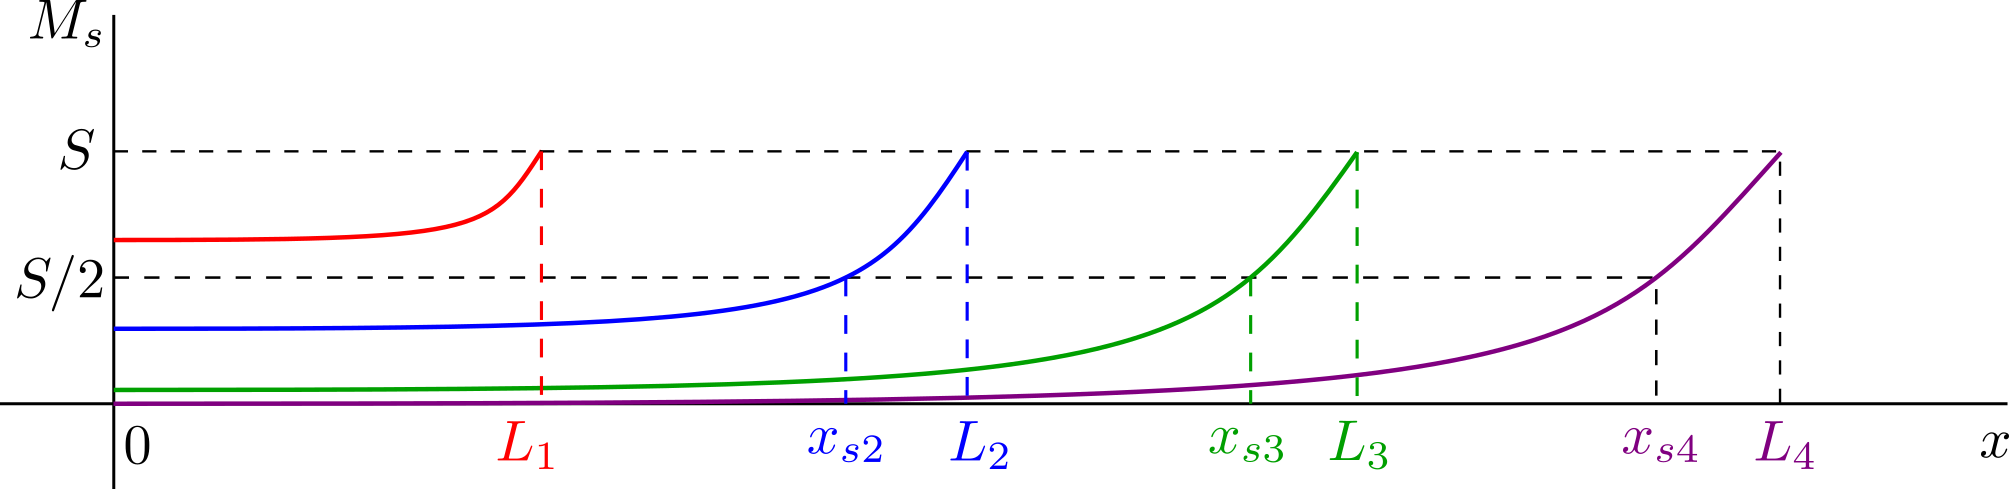
\includegraphics[width=\textwidth]{../../Pictures/Gradient_plot_growing.png}
\caption{\label{Gradient_plot_growing} Sketches of $M_s$ and $x_s$ on increasingly larger domains.}
\end{figure}
\item For the following question
\begin{enumerate}
\item For $L\gg 1$ we have that $\cosh\l L\sqrt{r/D}\r\approx \exp\l L\sqrt{r/D}\r/2$.
\item  Substituting this into the logarithmic form of $\cosh^{-1}$ we get
\bb
x_s=\sqrt{\frac{D}{r}}\cosh^{-1}\l\frac{1}{2}\cosh\l\sqrt{\frac{r}{D}}L\r \r\approx\ln\l \frac{\exp\l L\sqrt{r/D}\r}{4}+\sqrt{\l\frac{\exp\l L\sqrt{r/D}\r}{4}\r^2+1}\r.
\ee
Since $L\gg 1$
\bb
\sqrt{\l\frac{\exp\l L\sqrt{r/D}\r}{4}\r^2+1}\approx\frac{\exp\l L\sqrt{r/D}\r}{4}.
\ee
So
\bb
x_s\approx \sqrt{\frac{D}{r}}\ln\l\frac{\exp\l L\sqrt{r/D}\r}{2}\r\label{solxs}
\ee
\item Expanding the logarithm in \eqn{solxs} provides
\bb
x_s\approx \sqrt{\frac{D}{r}}\l \ln\l\frac{1}{2}\r+\ln\l\exp\l L\sqrt{r/D}\r\r \r,
\ee
which upon rearrangement and simplification gives
\bb
x_s\approx L- \sqrt{\frac{D}{r}}\ln\l 2\r.\label{Finalxs}
\ee
\end{enumerate}


\item Equation \eqref{Finalxs} tells us that $x_s$ does indeed increase as $L$ increases, it also tells us that $x_s$ is (to a first order approximation) a constant distance, $C=\sqrt{D/r}\ln\l 2\r$, away from the boundary $x=L$.

\item For large domains most of the cells are in form 1. Specifically, the only cells which see a concentration of morphogen above $S/2$ are those within the region $[L-C,L]$.

\item The plot can be seen in \fig{Exact_approximate}. We see that the approximation becomes excellent for $L\geq 6$ and the solution of $x_s$ disappears around  $L\approx 4$.
\begin{figure}[h!!!tb]
\centering
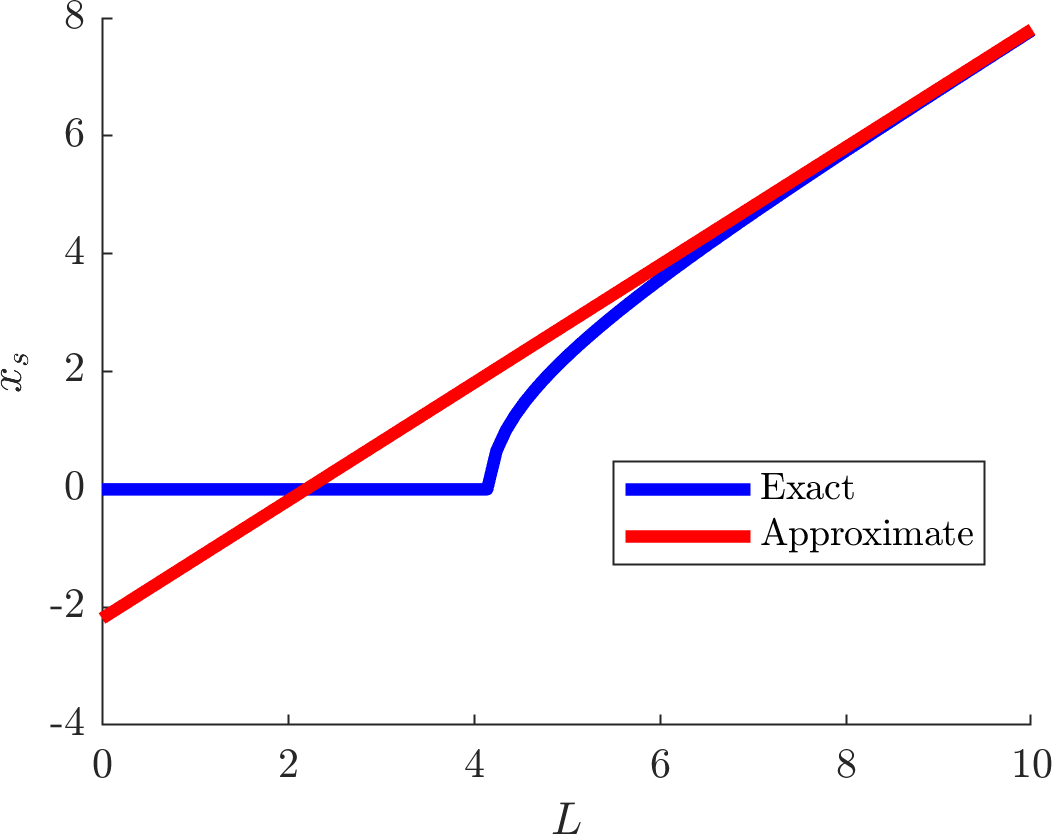
\includegraphics[width=\ttp]{../../Pictures/Exact_approximate.png}
\caption{\label{Exact_approximate} Comparing \eqns{xs}{Constant_diff}.}
\end{figure}
\end{enumerate}
\end{Answ}

\section{Patterning}
Alongside the Schnakenberg system, which we have seen throughout the course, the Gierer-Meinhardt kinetics\footnote{Meinhardt always maintained that the Schnakenberg system should be named after him and Gierer, as well, as it appeared as a specific case of one of their results in their original paper.} are a well-known system of morphogen kinetics that produce Turing patterns. 

The Gierer-Meinhardt reaction-diffusion system on a infinite one-dimensional domain is
\begin{align}
\D{A}{t}=&f(A,H)+ D_A \DD{A}{x},\label{GM1}\\
\D{H}{t}=&g(A,H)+ D_H \DD{H}{x},\label{GM2}
\end{align}
where
\begin{align}
f(A,H)=&\frac{\rho_1 A^2}{\l 1+KA^2\r H}-\mu_1 A,\\
g(A,H)=&\rho_2 A^2-\mu_2 H.
\end{align}
where $A$ and $H$ are the morphogen populations and $K, \rho_1, \rho_2, \mu_1, \mu_2, D_A$ and $D_H$ are positive constants. We assume that $A$ and $H$ remain finite over the domain and appropriate initial conditions are provided. \textbf{Initially, let us fix $\bm{K=0}$}.

As on sheet 2 this question is a good chance to practice deriving the Turing inequalities. However, if you are confident that you know what you are doing\footnote{Trust me, you don't.} then you can simply write down the required answers.
\begin{enumerate}
\item (0,0) is a homogeneous steady states of \eqns{GM1}{GM2}. What is the positive steady state, $(A_s,H_s)$?


\item Write down two inequalities that the positive steady state must satisfy in order to be stable, in the absence of diffusion.


\item Derive conditions under which the non-zero homogeneous steady state is stable in the absence of diffusion, but unstable when diffusion is included\footnote{As a personal hint I suggest keeping the system as $A_t=f(A,H)+D_A A_{xx}$ and $H_t=g(A,H)+D_H H_{xx}$, derive the inequalities in generality and then substitute the functional forms of $f$ and $g$ in at the end.} (\ie derive the Turing conditions).\label{Turing}


\setcounter{Counter1}{\value{enumi}}
\end{enumerate}

\textbf{Now assume that $\bm{K\neq0}$}. 
%The steady states can be defined as points all nullclines cross. So, hopefully, you have shown that in the quadrant $A\geq 0$ and $H\geq0$ there are two, (0,0) and one with both populations positive. In the previous question you may have drawn only one nullcline sketch. However, there are actually two situations. Namely, the non-zero steady state can either be before or after the maximum of the $A$ nullcline. 
\begin{enumerate}
\setcounter{enumi}{\value{Counter1}}
\item Show that the positive homogeneous steady state must satisfy
\bb
\frac{\mu_1\rho_2 A_s}{\rho_1\mu_2}(1+KA_s^2)=1.\label{Stst_criterion}
\ee

\item  Sketch the phase plane with nullclines $f=0$ and $g=0$ and demonstrate that there is still only one positive homogeneous steady state. Be sure to draw the two nullcline arrangements that can occur. Namely, the quadratic defined by $g=0$ can cut $f=0$ either before or after the maximum of $f=0$. Do not forget to add the directional arrows specifying the signs of $A_t$ and $H_t$.


\item What Jacobian sign structures are necessary for a Turing instability to take place?


\item Near the non-zero steady state the derivatives of $(A_t,H_t)$ change sign. Use the nullcline plot to extract the signs of $f_A, f_H, g_A$ and $g_H$ and, thus, show that a diffusion-driven instability can occur in only one of the two situations. Hint: in a $(A,H)$ phase plane the signs of  $f_A$ and $g_A$ are defined by changes in signs of $(A_t,H_t)$ along a horizontal path through $(A_s,H_s)$, whereas the signs of $f_H$ and $g_H$ are defined by changes in the signs of $(A_t,H_t)$ along a vertical path through $(A_s,H_s)$.
\end{enumerate}






\begin{Answ}
\subsection{Answers}
\begin{enumerate}
\item Since we are looking for homogeneous steady states of \eqns{GM1}{GM2}, $(A_s,H_s)$, we can ignore the spatial and temporal derivatives. Thus, the steady states are simultaneous solutions of $f(A_s,H_s)=g(A_s,H_s)=0$,
\begin{align}
0=&\frac{\rho_1 A_s^2}{ H_s}-\mu_1 A_s,\label{Stst1}\\
0=&\rho_2 A_s^2-\mu_2 H_s.\label{Stst2}
\end{align}
Ignoring the $(0,0)$ solution we can substitute \eqn{Stst2} into \eqn{Stst1} and derive
\bb
0=\frac{\rho_1\mu_2 A_s^2}{ \rho_2 A_s^2}-\mu_1 A_s,
\ee
which provides a value for $A$. Substituting this back into \eqn{Stst2} we are able to derive $H_s$. Thus, overall
\bb
(A_s,H_s)= \l \frac{\mu_2\rho_1}{\mu_1\rho_2}, \frac{\mu_2\rho_1^2}{\mu_1^2\rho_2}\r.
\ee


\item To derive the stability criterion we need to derive the Jacobian of $(f,g)$. This can be done by linearising around the positive steady state, \ie substitute
\bb
\l\begin {array}{c} A \\ H\end {array} \r=\l\begin {array}{c} \frac{\mu_2\rho_1}{\mu_1\rho_2} \\ \frac{\mu_2\rho_1^2}{\mu_1^2\rho_2} \end {array} \r+\l\begin {array}{c} \epsilon_1 \\ \epsilon_2\end {array} \r\exp(\lambda t)
\ee
into the spatially homogeneous version of \eqns{GM1}{GM2} and ignore quadratic and higher order terms of $\epsilon_1$ and $\epsilon_2$. We then finally derive conditions to ensure that  the real part of $\lambda$ is negative.

Alternatively, we can, straight away, write down the Jacobian
\bb
J(A,H)= \left[ \begin {array}{cc} 2\,{\frac {\rho_{{1}}A}{H}}-\mu_{{1}}&-{
\frac {\rho_{{1}}{A}^{2}}{{H}^{2}}}\\ \noalign{\medskip}2\,A\rho_{{2}}
&-\mu_{{2}}\end {array} \right] 
\ee
and evaluate it at the steady state
\bb
J(A_s,H_s)=  \left[ \begin {array}{cc} \mu_{{1}}&-{\frac {{\mu_{{1}}}^{2}}{\rho_{{
1}}}}\\ \noalign{\medskip}2\,{\frac {\mu_{{2}}\rho_{{1}}}{\mu_{{1}}}}&
-\mu_{{2}}\end {array} \right].
\ee
Once again, we can derive the eigenvalues, $\lambda$, of $J(A_s,H_s)$ and derive conditions under which the eigenvalues have negative real parts.

Alternatively,  we can check the notes in Appendix C and find that the stability criterion are
\begin{align}
0>&\text{trace}(J)=\mu_{{1}}-\mu_{{2}},\\
0<&\text{det}(J)=\mu_1\mu_2.
\end{align}

\item The first half of the problem (stability in the face of no diffusion) was done in the last question. Again you can either write the answers down from the notes, or derive them. Which is what we will do here. Since we are considering a spatial instability our perturbation is of the form
\bb
\l\begin {array}{c} A \\ H\end {array} \r=\l\begin {array}{c} A_s \\ H_s \end {array} \r+\l\begin {array}{c} \epsilon_1 \\ \epsilon_2\end {array} \r\exp(\lambda t)\cos(kx).\label{Spatial_perturbation}
\ee
Substituting perturbation \eqref{Spatial_perturbation} into \eqns{GM1}{GM2} provides
\begin{align}
\lambda\exp(\lambda t)\cos(kx)\l\begin {array}{c} \epsilon_1 \\ \epsilon_2\end {array} \r=&
-k^2\exp(\lambda t)\cos(kx)\l\begin {array}{cc} D_A & 0 \\ 0 & D_H\end {array} \r\l\begin {array}{c} \epsilon_1 \\ \epsilon_2\end {array} \r+\UB{\l\begin {array}{c} f(A_s,H_s) \\ g(A_s,H_s)\end {array} \r}{=0}\\
&+\exp(\lambda t)\cos(kx)\l\begin {array}{cc} f_A & f_H \\ g_A & g_H\end {array} \r\l\begin {array}{c} \epsilon_1 \\ \epsilon_2\end {array} \r.
\end{align}
Rearranging and simplifying gives
\bb
\l\begin {array}{c} 0 \\ 0 \end {array} \r=\l\begin {array}{cc} f_A-k^2D_A-\lambda & f_H \\ g_A & g_H-k^2D_H-\lambda\end {array} \r\l\begin {array}{c} \epsilon_1 \\ \epsilon_2\end {array} \r.
\ee
To have a non-trivial solution the matrix must have determinant zero,
\bb
0=\lambda^2-\lambda(f_A+g_H-k^2(D_H+D_A))+(f_A-k^2D_A)(g_H-k^2D_H)-f_Hg_A.
\ee
To have an instability there must be at least one solution, $\lambda$, with positive real part. Since
\bb
2\lambda_\pm=(f_A+g_H-k^2(D_H+D_A))\pm\sqrt{(f_A+g_H-k^2(D_H+D_A))^2-4((f_A-k^2D_A)(g_H-k^2D_H)-f_Hg_A)}
\ee
and we require $f_A+g_H<0$ for stability in the absence of diffusion then we know that 
\bb
f_A+g_H-k^2(D_H+D_A)<0
\ee
because $D_H+D_A>0$. Thus, the only way to get to ensure $\lambda_+>0$ is to enforce
\bb
0>(f_A-k^2D_A)(g_H-k^2D_H)-f_Hg_A=k^4D_AD_H-k^2(D_Ag_H+D_Hf_A)+f_Ag_H-f_Hg_A=h(k^2).
\ee
Since $h$ is a positive quadratic function in $k^2$ the only time it is negative is if there are two real, positive, roots:
\bb
2D_AD_Hk^2_\pm= D_Ag_H+D_Hf_A\pm\sqrt{(D_Ag_H+D_Hf_A)^2-4D_AD_H(f_Ag_H-f_Hg_A)}.
\ee
Thus, to ensure $k^2_\pm$ are real and positive we require that
\begin{align}
D_Ag_H+D_Hf_A>0&,\label{T1}\\
(D_Ag_H+D_Hf_A)^2-4D_AD_H(f_Ag_H-f_Hg_A)>0&,\label{T2}\\
f_Ag_H-f_Hg_A>0&.\label{T3}
\end{align}
Since we already require $f_Ag_H-f_Hg_A>0$ equations \eqref{T1} and \eqref{T3} can be wrapped up into
\bb
D_Ag_H+D_Hf_A>2\sqrt{D_AD_H(f_Ag_H-f_Hg_A)}.
\ee

Thus, finally, we can insert the functions $f$ and $g$ into the appropriate inequalities and specify that Turing patterns are generated when
\begin{align}
0>&\mu_{{1}}-\mu_{{2}},\\
0<&\mu_1\mu_2,\\
2\sqrt{D_AD_H\mu_1\mu_2}<&D_H\mu_{{1}}-D_A\mu_{{2}}.
\end{align}

\item Since we are looking for homogeneous steady states of \eqns{GM1}{GM2}, $(A_s,H_s)$, we can ignore the spatial and temporal derivatives. Thus, the steady states are simultaneous solutions of $f(A_s,H_s)=g(A_s,H_s)=0$,
\begin{align}
0=&\frac{\rho_1 A_s^2}{\l 1+KA_s^2\r H_s}-\mu_1 A_s,\label{Stst12}\\
0=&\rho_2 A_s^2-\mu_2 H_s.\label{Stst22}
\end{align}
Ignoring the $(0,0)$ solution we can substitute \eqn{Stst22} into \eqn{Stst12} and derive
\bb
0=\frac{\rho_1\mu_2 A_s^2}{\l 1+KA_s^2\r \rho_2 A_s^2}-\mu_1 A_s,
\ee
which upon further manipulation gives \eqn{Stst_criterion}.

\item The $A$ nullclines are 
\begin{align}
A=&0\label{NC1},\\
H=&\frac{\rho_1 A}{\l 1+KA^2\r \mu_1}.\label{NC2}
\end{align}
The $H$ nullcline is 
\begin{align}
H=&\frac{\rho_2}{\mu_2} A^2.\label{NC3}
\end{align}
The accompanying phase planes are shown in \fig{GM_phase_planes}. The figure demonstrates that there is one positive steady state.
\begin{figure}[h!!!tb]
\centering
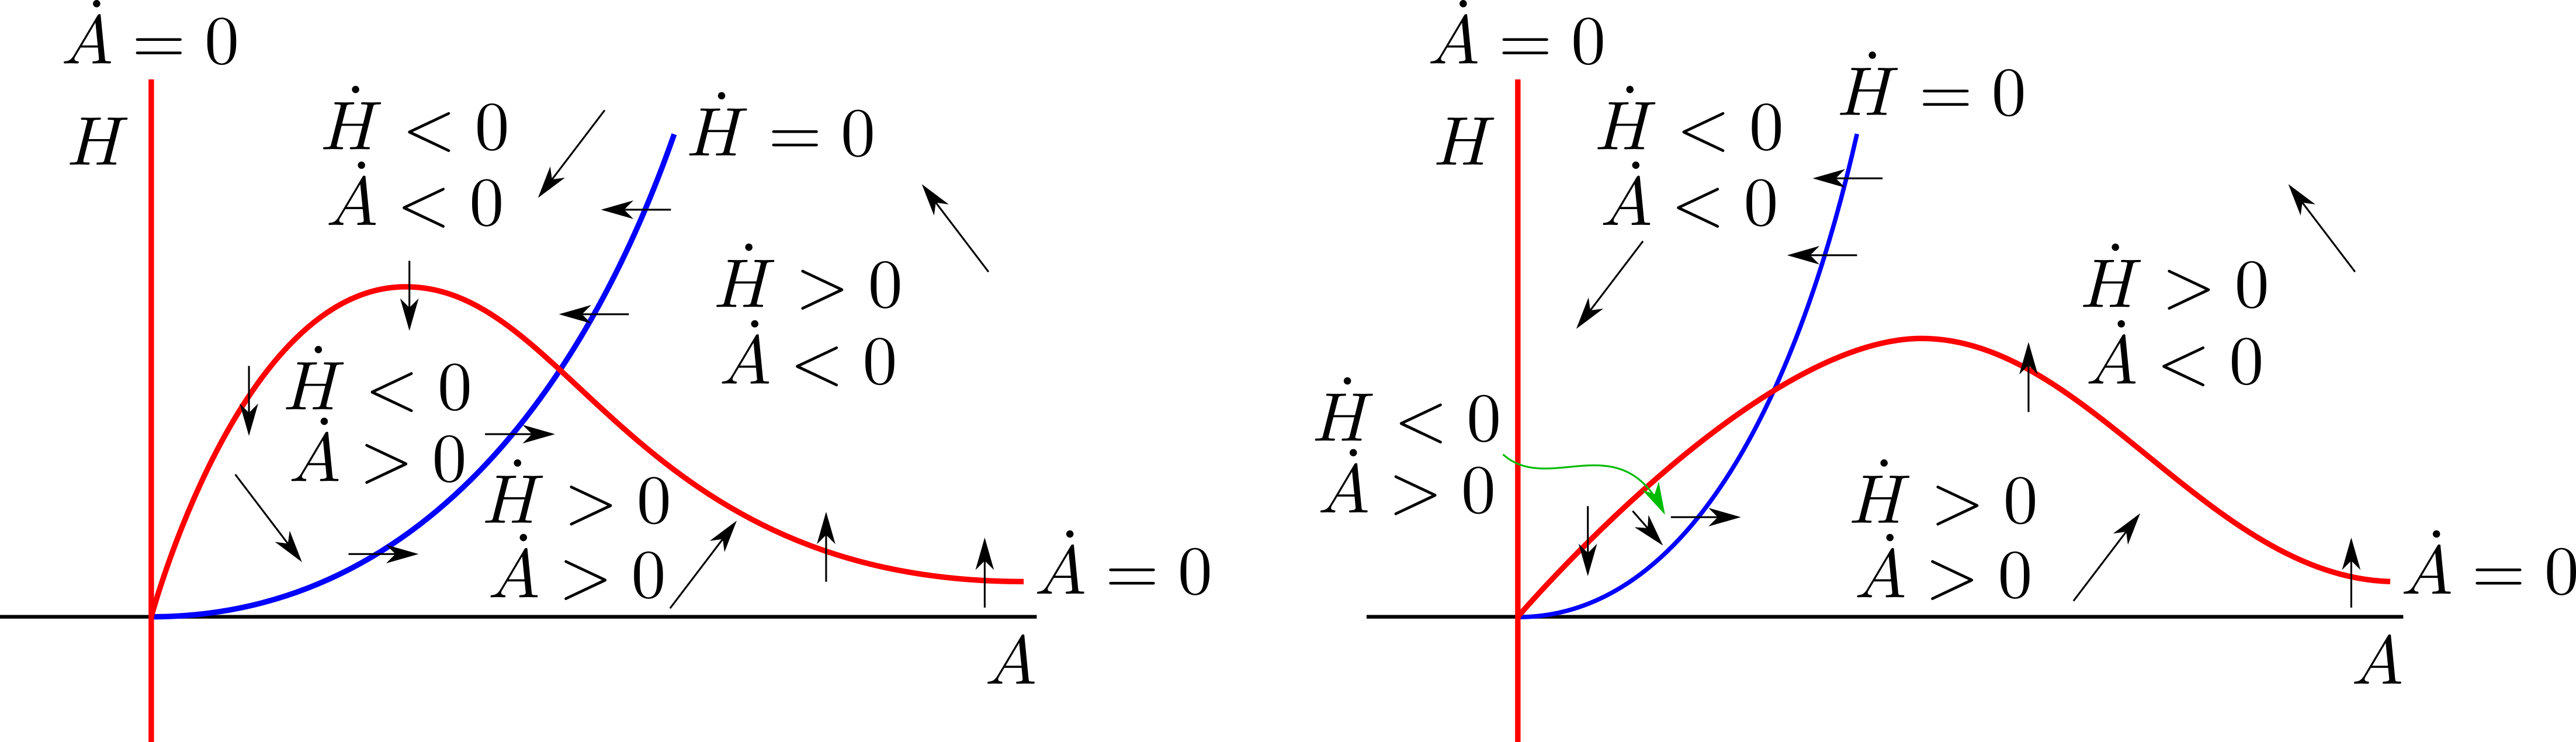
\includegraphics[width=\tp]{../../Pictures/GM_phase_planes.png}
\caption{\label{GM_phase_planes} The Gierer-Meinhardt phase planes.}
\end{figure}

\item Either from looking it up from the notes, or deriving it from question \ref{Turing}. The Jacobian must have the sign form
\bb
\left[ \begin {array}{cc} + & + \\ - & -\end {array} \right],\quad \textrm{ or }\quad\left[ \begin {array}{cc} + & - \\ + & -\end {array} \right]
\ee
along with column and row permutations.

\item Consider \fig{PP1} which shows the nullcline arrangement where $\dot{H}=0$ is to the right of the maximum of $\dot{A}=0$. Focus on the steady state and consider travelling along the dashed line from $x$ to $x'$. At $x$ $\dot{A}=f>0$ and at $x'$ $\dot{A}=f<0$, so as $A$ increases $\dot{A}=f$  goes from  positive to negative, so $\dot{A}=f$ must be a decreasing function of $A$ near the steady state. This means that $f_A<0$. Similarly at $x$, $\dot{H}=g<0$ and at $x'$, $\dot{H}=g>0$, so as $A$ increases $\dot{H}=g$  goes from negative to positive, so $\dot{H}=g$ must be an increasing function of $A$ near the steady state. This means that $g_A>0$. Following this logic along the vertical branch, from $y$ to $y'$ we discover that $f_H<0$ and $g_H<0$. Thus the accompanying Jacobian sign structure is
\bb
\left[ \begin {array}{cc} - & - \\ + & -\end {array} \right]
\ee
and, so, a Turing instability cannot happen.
\begin{figure}[h!!!tb]
\centering
\subfigure[\label{PP1}]{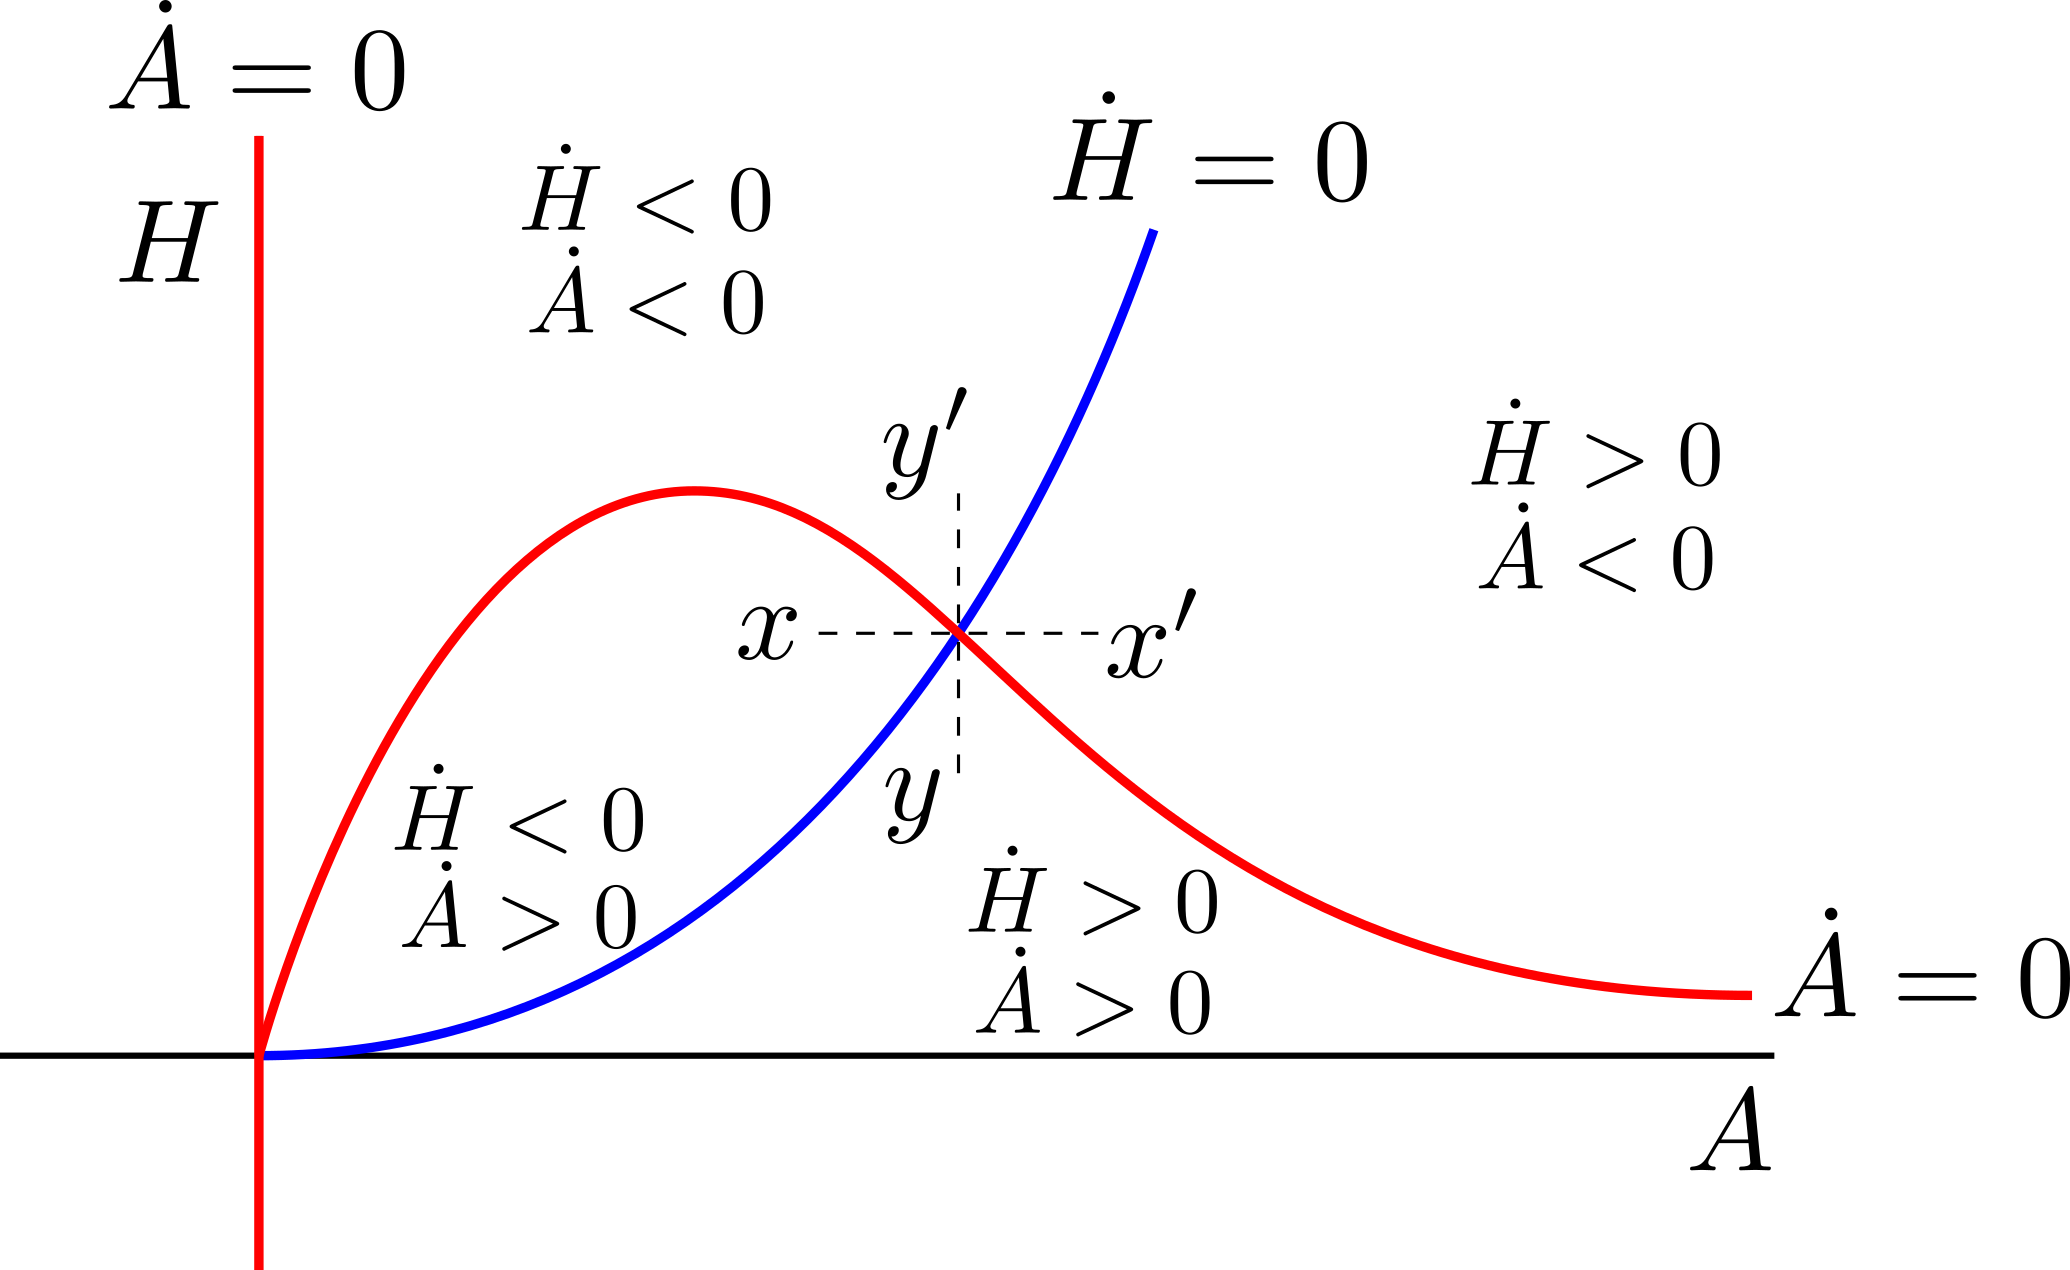
\includegraphics[width=\ttp]{../../Pictures/GM_phase_plane_derivative_1.png}}
\subfigure[\label{PP2}]{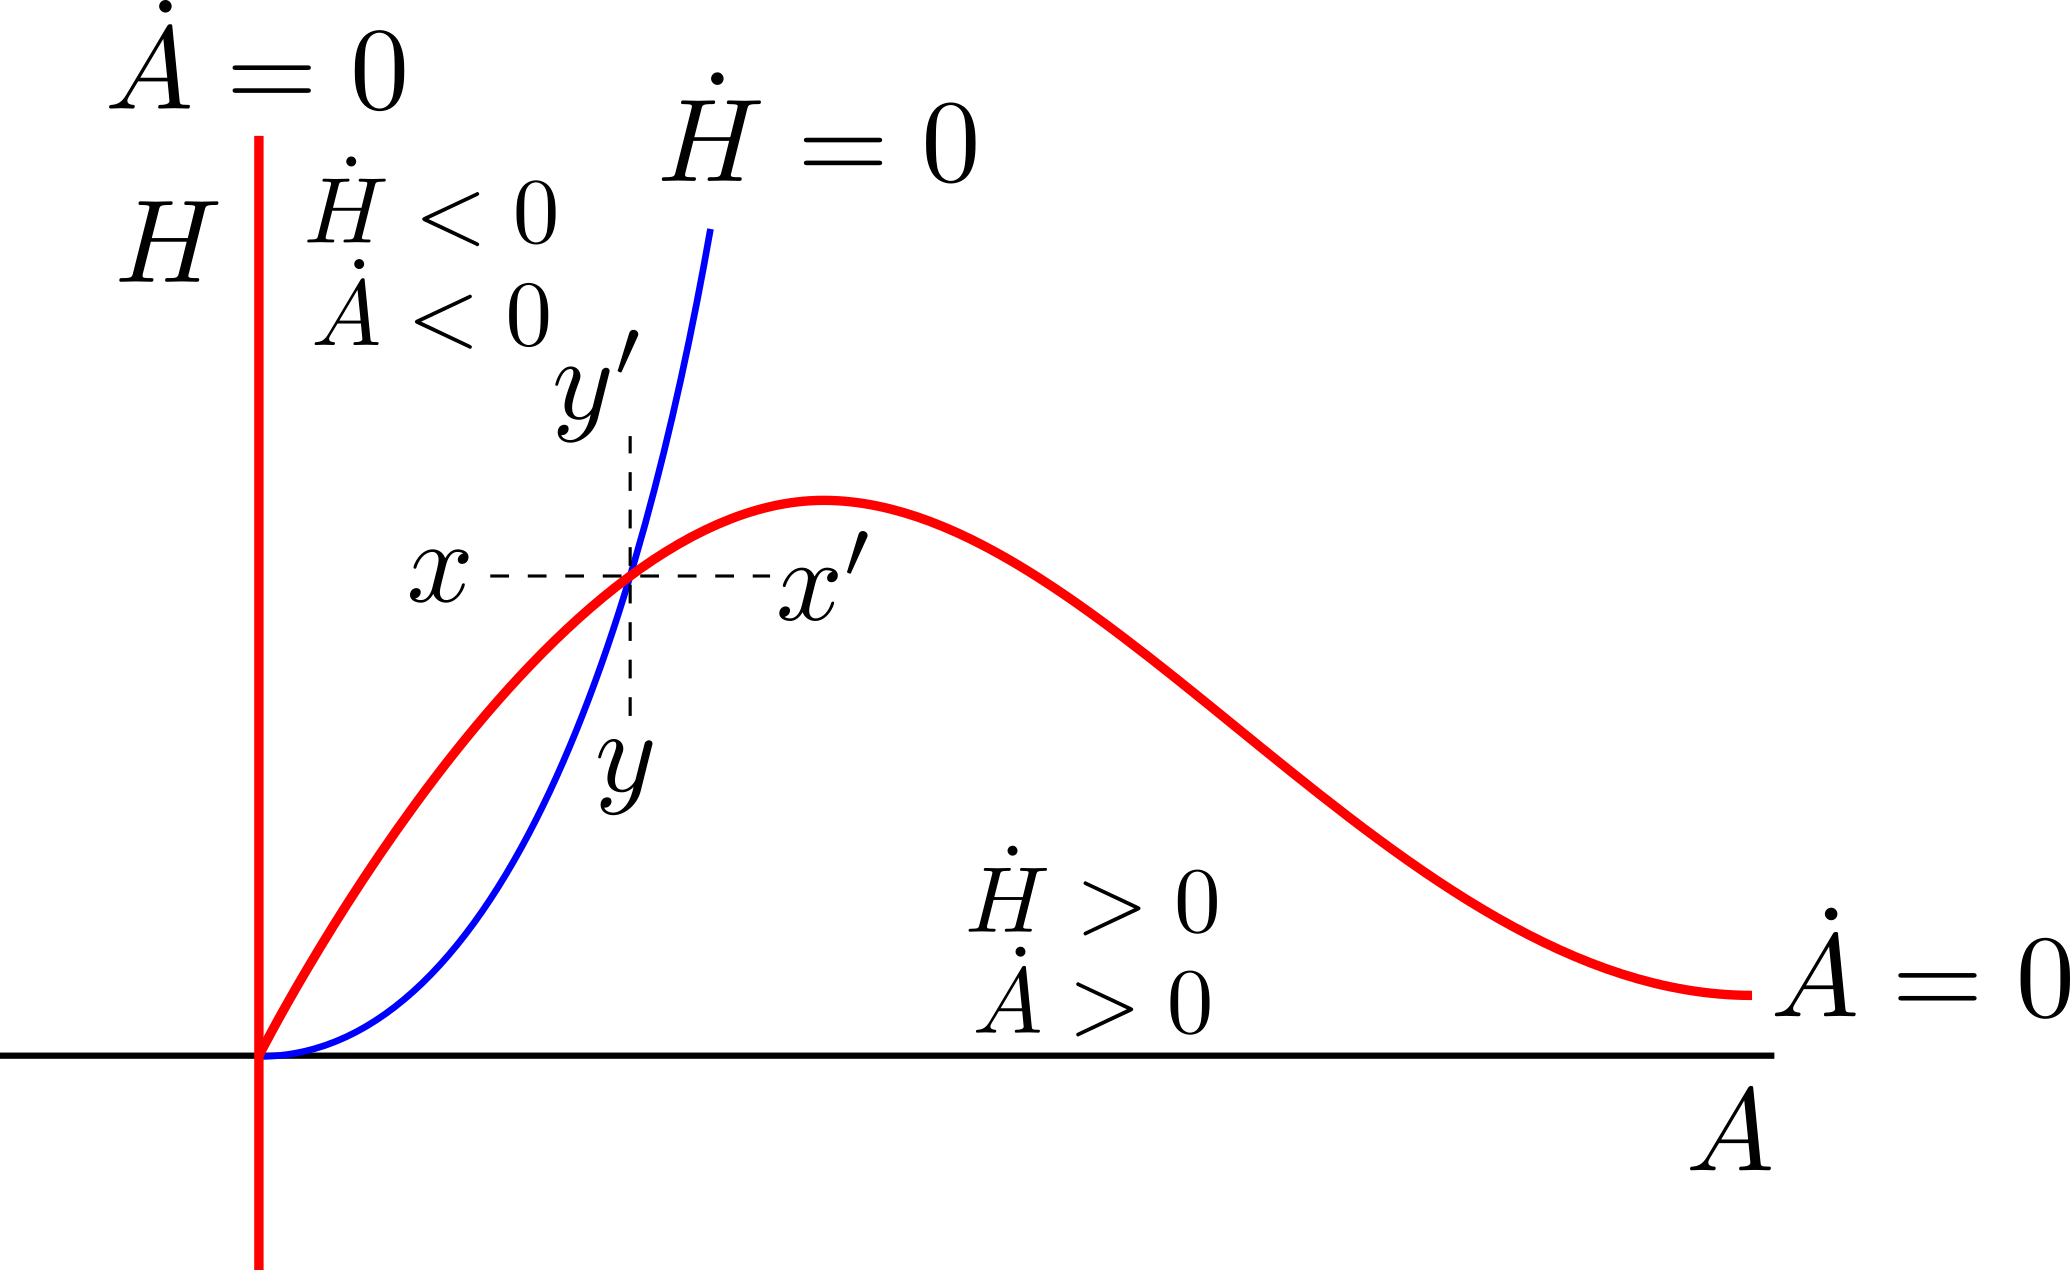
\includegraphics[width=\ttp]{../../Pictures/GM_phase_plane_derivative_2.png}}
\caption{\label{GM_phase_planes_derivatives} Extracting derivatives signs from the Geirer-Meinhardt phase planes.}
\end{figure}


If we now consider \fig{PP2} which shows the nullcline arrangement where $\dot{H}=0$ is to the left of the maximum of $\dot{A}=0$. We see that travelling from $x$ to $x'$ and $y$ to $y'$ only ever takes us between two sectors. The same logic applies and we can derive that $f_A>0$, $f_H<0$, $g_A>0$ and $g_H<0$. Thus the accompanying Jacobian sign structure is
\bb
\left[ \begin {array}{cc} + & - \\ + & -\end {array} \right]
\ee
and, so, a Turing instability could happen.

\end{enumerate}
\end{Answ}



\section{Simulating Turing patterns}
No Matlab this time. Simulating partial differential equations is not a simple task. However, there are websites out there that have done the heavy lifting for you.

The Gray-Scott reaction-diffusion model is
\begin{align}
&\D{u}{t}=D_u\nabla^2u -uv^2+F(1-u),\label{EGS1}\\
&\D{v}{t}=D_v\nabla^2v +uv^2-(F+k)v,\label{EGS2}
\end{align}
where appropriate boundary and initial conditions are assumed to be given and $D_u, D_v, F$ and $k$ are constants. $F$ is known as the feed rate as it causes more $u$ to be added to the system. $k$ is the death rate as it controls the rate at which $v$ is removed from the system.

You can play around with the feed rate, death rate and initial conditions through this \href{https://pmneila.github.io/jsexp/grayscott/}{online applet}. What patterns can you create? As a base level try and find spots, labyrinthine patterns and constantly evolving patterns, like those shown in \fig{Gray-Scott}. For those more adventurous try and find other patterns contained within these equations.
\begin{figure}[h!!!tb]
\centering
\subfigure[\label{GS1}]{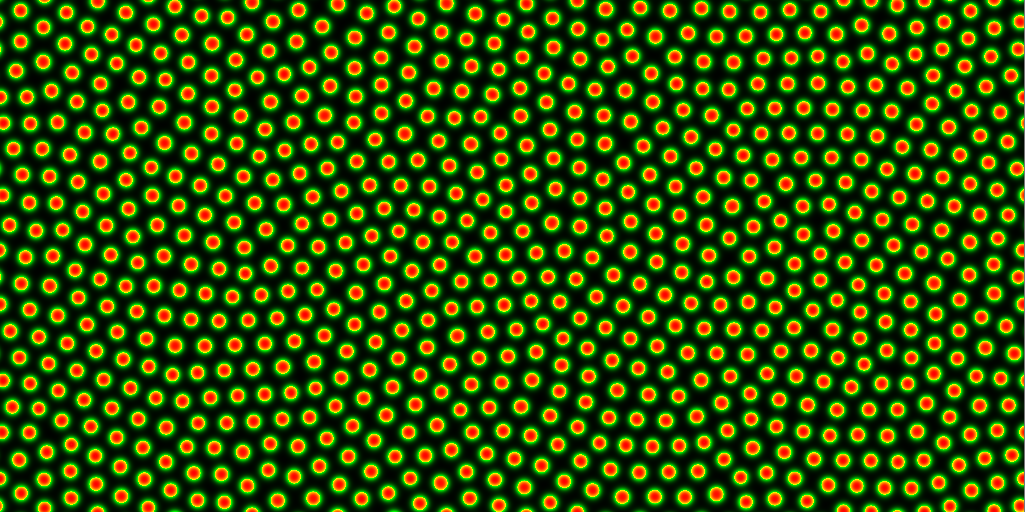
\includegraphics[width=\ttp]{../../Pictures/Spots_GS.png}}\\
\subfigure[\label{GS2}]{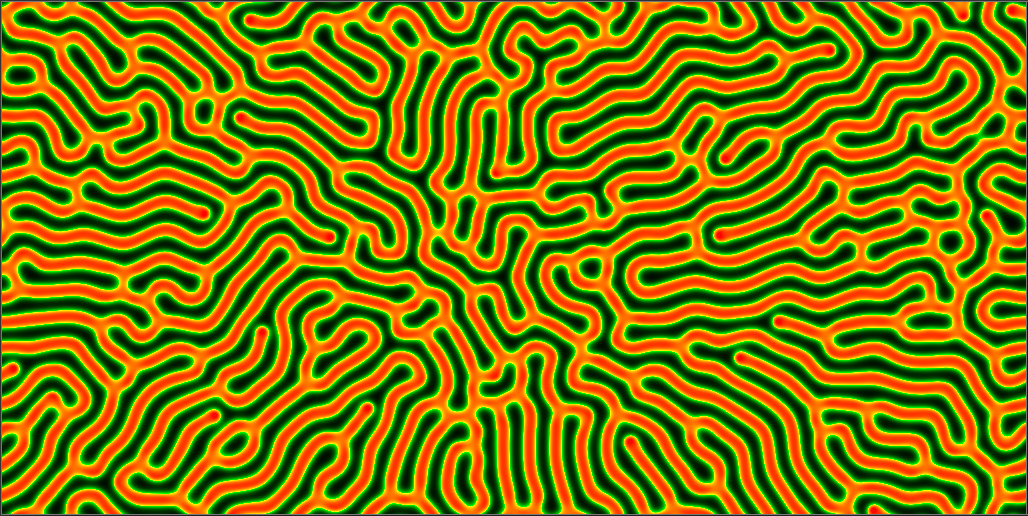
\includegraphics[width=\ttp]{../../Pictures/Labyrinthine_GS.png}}\\
\subfigure[\label{GS3}]{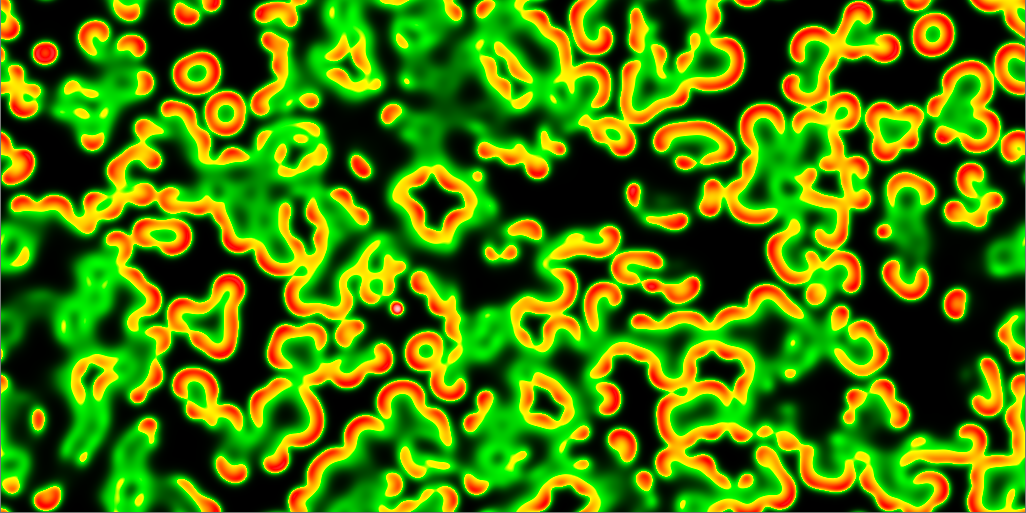
\includegraphics[width=\ttp]{../../Pictures/Chaotic_GS.png}}
\caption{\label{Gray-Scott} Possible patterns in the Gray-Scott \eqns{EGS1}{EGS2}.}
\end{figure}



\section*{Exam Revision}

\section{Properties of Turing patterns}
Consider a two species reaction-diffusion system with Neumann boundary conditions on a domain $B$, which has boundary $\partial B$,
\begin{align}
&\D{u}{t}=D_u\nabla^2u + f(u,v),\label{general1}\\
&\D{v}{t}=D_v\nabla^2v + g(u,v),\label{general2}\\
&\D{u}{n}=\D{v}{n}=0 \textrm{ on } \partial B.
\end{align}
 and random initial conditions. Further, assume that the kinetics and diffusion parameters are chosen such that the populations $(u,v)$ undergo  Turing patterning.
\begin{enumerate}
\item  Specify the Jacobian structures behind ``cross'' and ``pure'' kinetics.

\item  Explain why the resulting morphogen patterns of $(u,v)$ are in phase when pure kinetics are used and out of phase when cross kinetics are used. Note: \textit{in phase} means that the peaks and troughs of $u$ and $v$ occur at the same positions, where as \textit{out of phase} means that the peaks of $u$ correspond to the troughs of $v$ and vice-versa. Hint: consider the signs of $\epsilon_1$ and $\epsilon_2$. Under what conditions are they the same/different? What does this mean?

\item Explain why spatial oscillations can never occur at a Turing bifurcation point. Namely, show that the unstable eigenvalue $\lambda$ must always be real at the onset of patterning.

\item Why must $D_u\neq D_v$? (Hint: assume they are equal and derive a contradiction).
\end{enumerate}

\begin{Answ}
\subsection{Answers}
\begin{enumerate}
\item The ``cross'' kinetic Jacobian structure is
\bb
J=\left[ \begin {array}{cc} + & + \\ - & -\end {array} \right].
\ee
The ``pure'' kinetic Jacobian structure is
\bb
J=\left[ \begin {array}{cc} + & - \\ + & -\end {array} \right].
\ee
Note row and column permutations of the above are also valid.




\item We consider perturbations to the steady of the form
\bb
\l\begin {array}{c} u \\ v\end {array} \r=\l\begin {array}{c} u_s \\ v_s \end {array} \r+\l\begin {array}{c} \epsilon_1 \\ \epsilon_2\end {array} \r\exp(\lambda t)
\ee
where $\lambda$ is an eigenvalue of
\bb
J-Dk^2=\l\begin {array}{cc} f_u-k^2D_u & f_v \\  g_u & g_v-k^2D_v \end {array} \r
\ee
and
\bb
\bm{\epsilon}=\l\begin {array}{c} \epsilon_1 \\ \epsilon_2\end {array} \r
\ee
is a corresponding eigenvalue, thus,
\bb
(J-Dk^2)\bm{\epsilon}=\lambda \bm{\epsilon} \implies (J-Dk^2-\lambda I)\bm{\epsilon}=0.\label{Eig_eqn}
\ee
Consider the case of cross kinetics and write down the signs we know in the matrix $(J-Dk^2-\lambda I)$,
\bb
J-Dk^2-\lambda I=\l\begin {array}{cc} ? & + \\  - & - \end {array}\r.
\ee
Namely, the top right and bottom left entries are just $f_v$ and $g_u$, respectively, and, thus, do not change sign. The top left entry is positive (from $f_u$), but has values subtracted from it ($-k^2D_u-\lambda$), so we cannot guarantee its sign. However, the bottom right entry of $J$ is negative ($g_v<0$) in the case of cross kinetics and since we are subtracting further values from it, the bottom right term of $J-Dk^2-\lambda I$ remains negative.

Knowing these signs and that \eqn{Eig_eqn} must be satisfied we know that $\epsilon_1$ and $\epsilon_2$ must satisfy
\bb
\l\begin {array}{cc} s^?_1 & s^+_2 \\  s^-_3 & s^-_4 \end {array}
\r \l\begin {array}{c} \epsilon_1 \\ \epsilon_2\end {array} \r=0,\implies \begin {array}{c} s^?_1\epsilon_1+s^+_2\epsilon_2=0, \\  s^-_3\epsilon_1 + s^-_4\epsilon_2=0, \end {array}
\ee
where $s^i_j$ is some real number with sign $i$. The equation with unknown sign does not help. However, rearranging the other equation leads to
\bb
\frac{\epsilon_1}{\epsilon_2}=-\frac{s^-_3}{s^-_4}.\label{Signs}
\ee
Since $s^-_3$ and $s^-_4$ are both negative the right-hand side of  
\eqn{Signs} is negative, thus, we deduce that $\epsilon_1$ and $\epsilon_2$ must be of opposite sign. Finally, without loss of generality, let $\epsilon_1>0>\epsilon_2$ this means that the perturbation to $u_s$ is a positive cosine, whilst the perturbation to $v_s$ is a negative cosine and, thus, the patterns are out of phase.

The above logic can be followed with the pure kinetic sign structure. However, in this case you should derive that
\bb
\l\begin {array}{cc} s^?_1 & s^-_2 \\  s^+_3 & s^-_4 \end {array}
\r \l\begin {array}{c} \epsilon_1 \\ \epsilon_2\end {array} \r=0,\implies \begin {array}{c} s^?_1\epsilon_1+s^-_2\epsilon_2=0, \\  s^+_3\epsilon_1 + s^-_4\epsilon_2=0, \end {array}
\ee
resulting in
\bb
\frac{\epsilon_1}{\epsilon_2}=-\frac{s^+_3}{s^-_4}.\label{Signs2}
\ee
The right-hand sign on \eqn{Signs2} is positive, meaning that $\epsilon_1$ and $\epsilon_2$ are the same sign. Thus, the perturbations to the steady states are in phase.

\item The eigenvalues of the Turing instability are
\bb
2\lambda_\pm=(f_u+g_v-k^2(D_u+D_v))\pm\sqrt{(f_u+g_v-k^2(D_v+D_u))^2-4((f_u-k^2D_u)(g_v-k^2D_v)-f_vg_v)}.
\ee
These are imaginary if and only if
\bb
(f_u+g_v-k^2(D_v+D_u))^2-4((f_u-k^2D_u)(g_v-k^2D_v)-f_vg_v)<0 \label{Imag}
\ee
However, $(f_u+g_v-k^2(D_v+D_u))^2>0$ and for an instability to exist we need $-4((f_u-k^2D_u)(g_v-k^2D_v)-f_vg_v)>0$. Thus, at the onset of patterning inequality \eqref{Imag} cannot be satisfied and, thus, $\lambda_\pm$ are real, so oscillations in time do not happen.

\item Two of the Turing inequalities are
\begin{align}
&f_u+g_v<0\\
&D_vf_u+D_ug_v>0.\label{DD}
\end{align}
If $D_v=D_u>0$ then we could factor the constant out of \eqn{DD} and, thus, be able to derive
\begin{align}
&f_u+g_v<0\\
&f_u+g_v>0,
\end{align}
resulting in a contradiction.


\end{enumerate}
\end{Answ}


\section{Creating the model}
For each of the following images in \fig{q1-3} write down a set of reaction-diffusion equations that could provide the images as a steady state solution. Do not forget to provide boundary conditions. For initial conditions assume that there is a small spatially random amount of morphogen throughout the domain. 
\begin{figure}[h!!!tb]
\centering
\subfigure[\label{q1}]{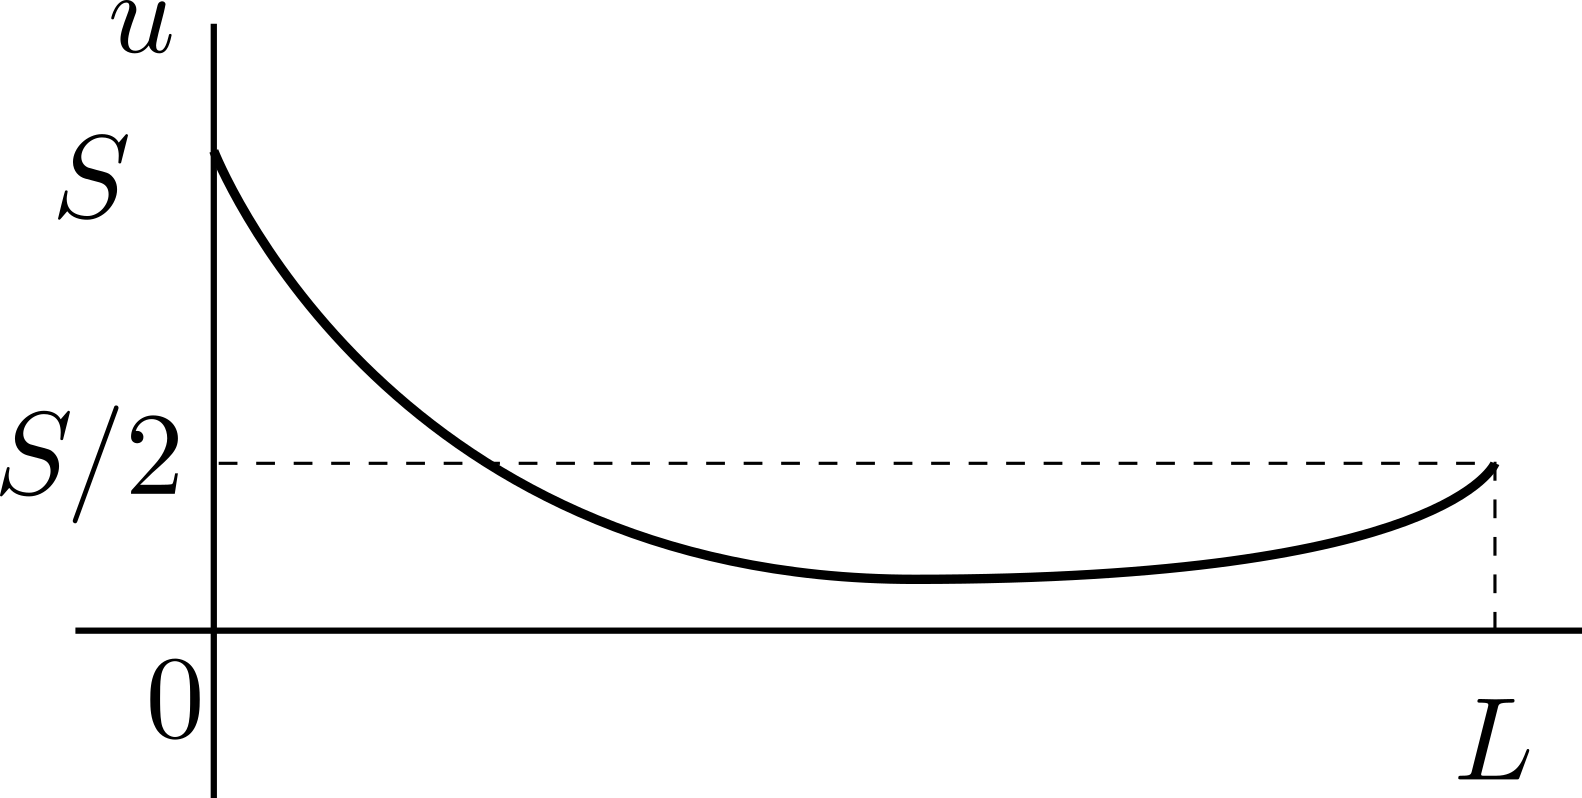
\includegraphics[width=\tttp]{../../Pictures/PDE_q1.png}}
\subfigure[\label{q2}]{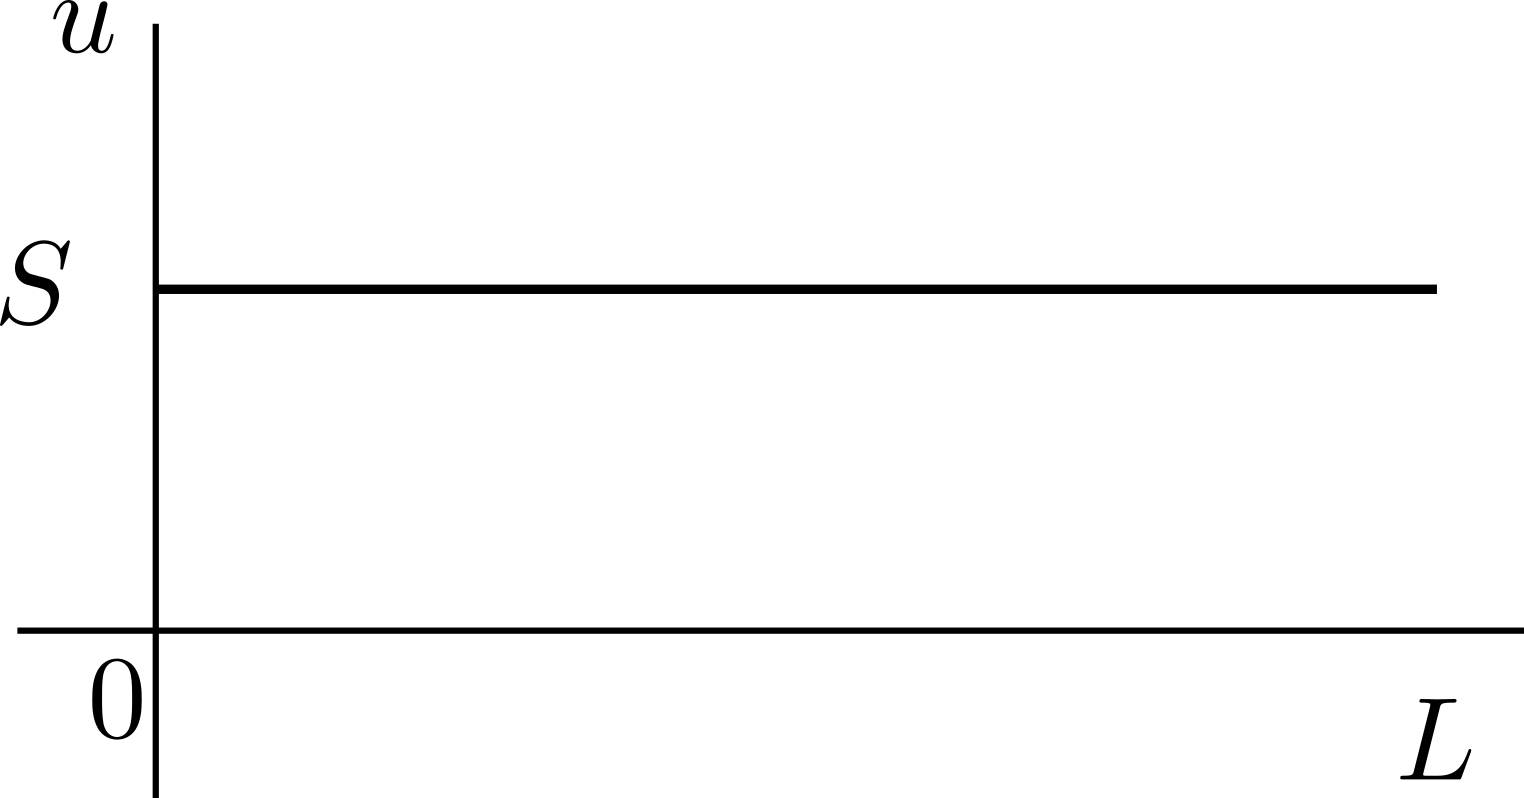
\includegraphics[width=\tttp]{../../Pictures/PDE_q2.png}}
\subfigure[\label{q3}]{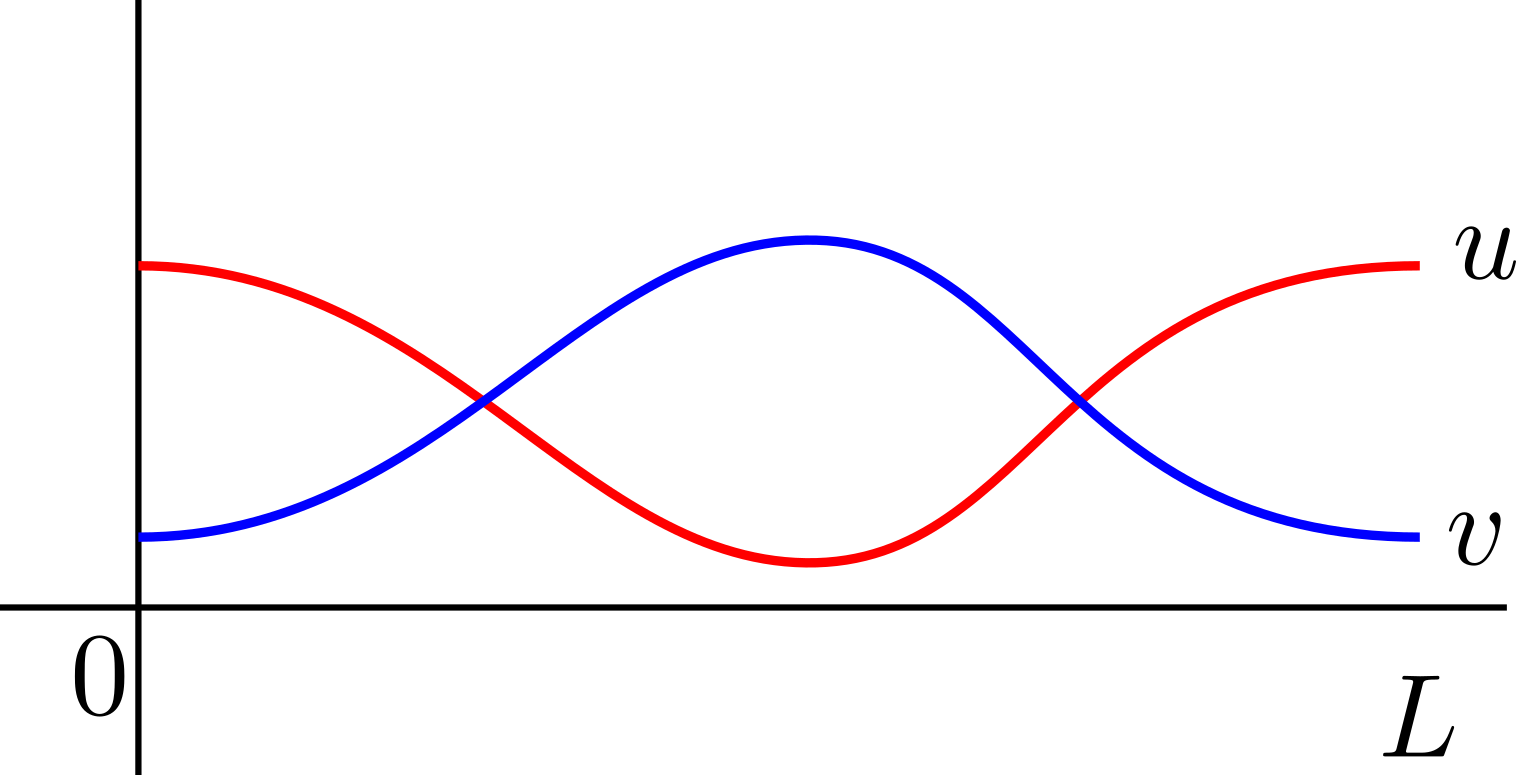
\includegraphics[width=\tttp]{../../Pictures/PDE_q3.png}}
\caption{\label{q1-3} Three steady state morphogen profiles.}
\end{figure}


\begin{Answ}
\subsection{Answers}
Note that the following suggestions are non-unique (as illustrated in case 2), so if you have a different suggestion you could be right.
\begin{enumerate}
\item Things to notice:
\begin{itemize}
\item the boundaries are fixed to two different values;
\item the profile of $u$ decays away from the boundaries.
\end{itemize}
Using these two pieces of information the follow reaction-diffusion equation should give a steady profile similar to \fig{q1}, for appropriate values of $D$ and $\gamma$.
\bb
\D{u}{t}=D\DD{u}{x}-\gamma u,
\ee
\bb
u(0,t)=S, \quad u(L,t)=S/2.
\ee

\item Since the entire profile is flat the boundaries could either be fixed at $S=0$, or they could be zero-flux. One potential equation behind this system is:
\bb
\D{u_1}{t}=D\DD{u_1}{x},
\ee
\bb
u_1(0,t)=S, \quad u_1(L,t)=S.
\ee
Another potential is
\bb
\D{u_2}{t}=D\DD{u_2}{x}+ru_2(S-u_2),
\ee
\bb
\D{u_2}{x}(0,t)=0=\D{u_2}{x}(L,t).
\ee

\item We note that the steady state is a combination of two heterogeneous morphogens that are out of phase. This suggests using a reaction-diffusion system. Equally, the morphogen profile at the boundaries is `flat', which suggests zero-flux boundary conditions. Hence, we need a system of the following form
\begin{align}
&\D{u}{t}=D_u\D{u}{x}+f(u,v),\\
&\D{v}{t}=D_v\D{v}{x}+g(u,v),
\end{align}
\bb
\D{v}{x}(0,t)=\D{u}{x}(0,t)=0=\D{u}{x}(L,t)=\D{v}{x}(L,t),
\ee
such that $f$ and $g$ satisfy the Turing instability inequalities (see \eqns{T1}{T3}). Additionally, because the populations are out of phase we know that the Jacobian of partial derivatives must satisfy the cross kinetic pattern,
\bb
J=\left[ \begin {array}{cc} + & + \\ - & -\end {array} \right].
\ee
If you had gotten this far I would be happy with this answer. However, pushing your memory a little further you might remember that the Schnakenberg kinetics are Turing unstable and produce out of phase patterns and, thus, would make a satisfactory choice for $f$ and $g$.
\end{enumerate}

\end{Answ}



\end{document}